\documentclass[10pt]{article}

% Required packages
\usepackage{bm,bbm}
\usepackage{amsmath,amssymb,amsthm,cancel}
\usepackage{algorithm, algpseudocode}
\usepackage{minted, caption}



% Color references
\usepackage[
    colorlinks=true, citecolor=green, linkcolor=blue]{hyperref}

\newcommand{\homework}[2]{
	\noindent
    \begin{center}
    	\framebox{
        	\vbox{
            	% Course Title and Date
            	\hbox to \hsize { \textsc{ORIE 7390 - Special Topics in
				Mathematical Programming} \hfill \textsc{#1} }
                \vspace{4mm}
                % Title of handout/homework
                \hbox to \hsize { {\Large \hfill \textsc{#2} \hfill} }
                \vspace{1mm}
            }
        }
    \end{center}
}

\newenvironment{alglist}{\begin{list}{}{\setlength{\leftmargin}{1.5cm}
\setlength{\rightmargin}{0cm}\setlength{\itemsep}{1ex}\setlength{\parsep}{1ex}}}{\end{list}}

\newcommand{\problem}[3]
{\fbox{\parbox{6in}{{\bf #1}\begin{itemize}\item{\bf Input:} {#2} \item{\bf Goal:} {#3}\end{itemize}}}}

\usepackage{latex-macros}
\usepackage{todonotes}
\usepackage{tikz,pgfplots}
\pgfplotsset{compat=1.12}
\usepackage{algorithm, algpseudocode}
\usepackage[margin=1in]{geometry}
\usetikzlibrary{shapes.geometric}
%\usepackage{parskip}
\usepackage[capitalize]{cleveref}
\usepackage{exercise}
\usepackage{svg}

\usepackage{todonotes}

\newcommand{\regdiff}{\hat{\partial}}
\newcommand{\bd}[1]{\mathrm{bd}\left( #1 \right)}

\begin{document}

\allowdisplaybreaks
\everymath{\displaystyle}

\homework{Vasileios Charisopoulos}{Homework 1}{vc333}

\vspace{1em}
\begin{Exercise}
	\label{ex:p1}
	Consider $f(u, v) = \abs{u} + v^2$, so $\dom f = \Rbb^2$. This function is
    easily shown to be convex as a sum of convex functions, which will be
    needed in the sequel. Additionally, it is proper by virtue of being bounded
    below from $0$, with minimum value $\min f = f(0, 0) = 0$, and closed since
    its individual summands are also closed.

    \paragraph{1.}
        In class, we mentioned the theorem given by Brezis: for closed, convex,
        proper $f$ which attain their minima, there exist unique steepest
        descent trajectories $X(\cdot)$ which satisfy
        \begin{align}
            \begin{cases}
                X(0) = x_0 = \begin{pmatrix} 1 \\ 1 \end{pmatrix}, & \\
                \frac{\dd{} X(t)}{\dd t} \in -\partial f(X(t)), & \text{a.e.}
            \end{cases}
            \label{eq:descent_trajectory}
        \end{align}
        Observe that $f$ is separable, which means that we may treat each
        coordinate of the descent trajectory separately, as seen below:
        \begin{align*}
            \left\{
            \begin{aligned}
                \frac{\dd{} X_1(t)}{\dd t} & \in
                -\partial \abs{X_1(t)} \\
                \frac{\dd{} X_2(t)}{\dd t} & \in
                -2 X_2(t)
            \end{aligned} \right.
        \end{align*}
        The second of the above ODEs is easy to solve, since the inclusion is
        actually an equality giving us (using dot notation for the time
        derivative):
        \[
            \dot{X}_2(t) + 2 X_2(t) = 0 \Rightarrow
            X_2(t) = e^{-2t} X_2(0) = e^{-2t}.
        \]
        For the other part, we have
        \[
            \dot{X}_1(t) + \partial \abs{X_1(t)} = 0,
        \]
        where we have to take cases depending on $X_1(t)$'s sign:
        \begin{itemize}
        \item $X_1(t) > 0$: in that case, we have $\dot{X}_1(t) = -1 \Rightarrow
            X_1(t) = C - t = 1 - t$, since $X_1(0) = 1$.
        \item $X_1(t) = 0$: in that case, we must have $\dot{X}_1(t) =
            0 = \partial^{\circ} f(X_1(t))$, which is the minimum length
            subgradient, This means that if we start from $X(0)$ and eventually
            hit $X(t)$ such that $X_1(t) = 0$, $X_1(s) = 0, \; \forall s \geq
            t$.
        \item $X_1(t) < 0$: this case implies that
            $\dot{X}_1(t) = 1 \Rightarrow X_1(t) = t + C$, but $t \in \Rbb_+$
            so we will end up in $X_1(0) = 0$ before we get any chance to reach
            $X_1(t) < 0$.
        \end{itemize}
        Putting all of the above together, we recover
        \[
            X(t) = \begin{pmatrix}
                    \max(1 - t, 0) \\
                    e^{-2t}
                \end{pmatrix}
        \]

    \paragraph{2.}
		Let us simplify the notation by dropping $\lambda$ from $x_k^{\lambda}$
		for now, until we determine the solution of the proximal map.
		Consider $x^* = \argmin_{x} f(x) + \frac{\lambda}{2} \norm{x - x_k}^2$.
		Since $f$ is a convex function, the proximal map is well defined and,
		additionally, based on $f$ having full domain, we can conclude that
		\[
			\partial \left(f(x) + \frac{\lambda}{2} \norm{x - x_k}^2 \right)
			= \partial f(x) + \partial \left( \frac{\lambda}{2} \norm{x -
			x_k}^2 \right).
		\]
		Therefore we simply have to write the first-order optimality conditions
		for $x^*$, which means that
		\begin{align*}
			0 &\in \partial f(x^*) + \lambda ( x^* - x_k ) \Rightarrow
			0 \in \begin{pmatrix} \partial \abs{x^*_1} \\ 2 x^*_2 \end{pmatrix}
				+ \lambda \begin{pmatrix} x^*_1 - x_k^{(1)} \\ x^*_2 - x_k^{(2)}
				\end{pmatrix},
		\end{align*}
		which we arrived at observing that the function minimized is separable.
		For the smooth part, trivial algebraic manipulations lead to $x_2^* =
		\frac{\lambda}{2 + \lambda} x_k^{(2)}$. For the nonsmooth part, we
		know from ORIE 6328 that the solution is given by the
		\textit{soft thresholding} operator. Nevertheless, we repeat the
		derivation to convince the reader. Consider the following cases:
		\begin{enumerate}
			\item $x^*_1 > 0$: in that case $\partial \abs{x_1}^* = 1$ and
				$x_k^{(1)} = x_1 + \frac{1}{\lambda}$.
			\item $x^*_1 < 0$: like before, we have $\partial \abs{x_1}^* = -1$
				leading to $x_k^{(1)} = x_1 - \frac{1}{\lambda}$.
		\end{enumerate}
		The two cases above imply that $\sign(x_k^{(1)}) = \sign(x_1^*)$ when
		$x_1^* \neq 0$. Now, consider the case where it is equal to $0$. We
		know from convex analysis that $\partial \abs{x} = [-1, 1]$ when
		$x = 0$, so $x_k^{(1)}$ must be $\in \frac{[-1, 1]}{\lambda}$. Gathering all the
		cases above (and keeping in mind that $\lambda > 0$) gives us
		\begin{align*}
			x_1^* &= \sign(x_k^{(1)}) \max\left(\abs{x_k^{(1)}} -
				\frac{1}{\lambda}, 0\right).
		\end{align*}
		Therefore, we have
		\[
			x_{k+1}^{\lambda} = \begin{pmatrix}
				\sign(x_k^{(1)}) \max\left( \abs{x_k^{(1)}} -
				\frac{1}{\lambda}, 0 \right) \\
				\frac{\lambda}{2 + \lambda} x_k^{(2)}
			\end{pmatrix}, \; \forall \lambda > 0.
		\]

    \paragraph{3.}
		We provide code that computes the proximal point sequence and saves the
        resulting trajectory in a \texttt{.csv} file as a \texttt{Python}
        script, which is attached in a \texttt{.zip} file along with this
        report. Example sequences as well as the real trajectory can be found
		in~\cref{fig:prox-seq}.
		\begin{figure}[h]
			\centering
            \begin{tikzpicture}% table
            \begin{axis}[xlabel=$x$,ylabel=$y$, legend pos=north west,
                         legend style={nodes={scale=0.75}}]
            \addplot+[mark options={scale=0.75}] table[x=x,y=y, col
            sep=comma] {code/prox_50.000.csv};
            \addplot+[mark options={scale=0.75}] table[x=x,y=y, col
            sep=comma] {code/prox_20.000.csv};
            \addplot+[mark options={scale=0.75}] table[x=x,y=y, col
            sep=comma] {code/prox_5.000.csv};
            \addplot+[no markers, thick] table[x=x,y=y, col
            sep=comma] {code/trajectory_10.000.csv};
            \legend{$\lambda = 50$, $\lambda = 20$, $\lambda=5$, Real};
            \end{axis}
            \end{tikzpicture}
            \caption{Proximal point sequence for different $\lambda$
            against real trajectory}
            \label{fig:prox-seq}
		\end{figure}
        The real trajectory plotted is $x(t), 0 \leq t \leq 10$.

    \paragraph{4.}
        Results presented in lecture suggest that $\lim_{k \to \infty}
        x_{k}^{k/t} \to x(t)$. Let us try to see if we can verify this result
        analytically for our proximal step sequences. First, examine the
        second coordinate, for which it holds
        \[
            v_{k} := {(x_{k+1}^{\lambda})}_2 = \frac{\lambda}{2 +
            \lambda} x_k^{(2)}
        \]
        If we substitute $x^{(2)}_0 = 1$ we obtain
        \( v_k = \left( \frac{\lambda}{2 + \lambda} \right)^{k} \)
        and substituting $\lambda = \frac{k}{t}$ gives us
        \begin{align*}
            \left( \frac{\lambda}{2 + \lambda} \right)^k &=
                \left( \frac{k/t}{2 + k/t} \right)^k =
                \left( \frac{k}{2t + k} \right)^k =
                \left(1 - \frac{\alpha}{k + \alpha}\right)^k \\
            \Rightarrow \lim_{k \to \infty} v_k &= e^{-\alpha},
        \end{align*}
        where in our case we set $\alpha = 2t$. Therefore,
        \( \lim_{k \to \infty} \left( x_{k}^{k/t} \right)_2 = e^{-2t} = x_2(t)
        \).
        The case for $x_1$ is a bit more delicate. Notice that the initial point
        $x_0^{(1)} = 1$ provides us with the first iterate
        \( u_1 := \left( x^{\lambda}_{1} \right)_1 =
           \max\big(1 - \frac{1}{\lambda}, 0\big) \).
        Then, assuming that $\lambda > 1$, which implies that $\frac{1}{\lambda}
        < 1$, we obtain:
        \(
            u_2 = \max\bigg( \abs{1 - \frac{1}{\lambda}} - \frac{1}{\lambda}, 0
            \bigg) = \max\bigg( 1 - \frac{2}{\lambda}, 0 \bigg).
        \)
        Notice that the above gives us a decreasing sequence of positive $u_k$'s
        until the first point where we hit some $u_{p} < \frac{1}{\lambda}$,
        which will give us $\max\left(u_p - \frac{1}{\lambda}, 0\right) = 0$.
        Therefore, we obtain
        \[
            u_k = \max\left(1 - \frac{k}{\lambda}, 0\right)
            \overset{\lambda=\frac{k}{t}}{\Rightarrow} u_k
            = \max\left(1 - t, 0\right) \Rightarrow
            \lim_{k \to \infty} u_k = \max(1 - t, 0) = x_1(t).
        \]
        Note that our assumption $\lambda > 1$ is without loss of generality,
        since taking the limit $k \to \infty$ results in a ratio $\frac{k}{t} >
        1$ for all finite values of $t$.
\end{Exercise}

\vspace{1em}

\begin{Exercise}
	\label{ex:p2}
	Consider $f: \Rbb^n \to \Rbb$, continuously differentiable. This means that
	$f$ satisfies, at any point $x$:
	\begin{align}
		f(x + d) &= f(x) + \ip{\grad f(x), d} + o(d), \;
		\lim_{d \to 0} \frac{o(d)}{\norm{d}} = 0.
		\label{eq:diff-defn}
	\end{align}
	First, consider $x$ being a minimizer. Then, we have defined the slope to
	be $0$ by convention, which agrees with the first-order condition $\grad
	f(x) = 0$ in unconstrained optimization. The nontrivial case has $x$ not
	being a minimizer.

	Let us work with the definition of the slope. We write
	\begin{align*}
		\abs{\grad f}(x) &= \limsup_{z \to x} \frac{f(x) - f(z)}{\norm{x - z}}
		= \lim_{\delta \dto 0} \sup_{\norm{z - x} \leq \delta} \frac{f(x) -
		f(z)}{\norm{x - z}} \\
			&= \lim_{\delta \dto 0} \sup_{\norm{d} \leq \delta}
			\frac{f(x) - f(x + d)}{\norm{d}} =
				\lim_{\delta \dto 0} \sup_{\norm{d} \leq \delta}
			\frac{f(x) - f(x) - \ip{\grad f(x), d} + o(d)}{\norm{d}} \\
			&\overset{(\text{Cauchy-Schwarz})}{\leq} \limsup_{d \to 0} \left(
				\frac{\norm{\grad f(x)} \norm{d}}{\norm{d}} +
			  	\frac{o(d)}{\norm{d}} \right) = \norm{\grad f(x)},
	\end{align*}
	where we used the fact that $\frac{o(d)}{\norm{d}} = 0$ as $d \to 0$.
	It is left to show that $\abs{\grad f}(x) \geq \norm{\grad f(x)}$, and the
	proof will be complete. To that end, observe that since $z \to x$ in the
	limit superior of $\abs{\grad f}$'s definition, we must have for any
	$d \in \ball_2$:
	\[
		\abs{\grad f}(x) \geq \lim_{t \to 0} \frac{f(x) - f(x + td)}{t},
	\]
	which is simply the mathematical way to state the fact that approaching $x$
	by arbitrary trajectories can only give us a bigger $\sup$ than by
	approaching it from a single direction. Then, setting $d = -\frac{\grad
	f(x)}{\norm{\grad f(x)}}$ and replacing $f(x + td)$ by~\cref{eq:diff-defn}
	gives us:
	\begin{align*}
		\abs{\grad f}(x) &\geq
		\lim_{t \dto 0} \frac{f(x) - f(x) + t \norm{\grad f(x)} + o(t)}{t}
			= \norm{\grad f(x)},
	\end{align*}
	which completes the claim. Hence $\abs{\grad f}(x) = \norm{\grad f(x)}$
	when $f$ is $C^1$.
\end{Exercise}

\vspace{1em}

\begin{Exercise}
	\label{ex:p3}
	Consider $f: \Rbb^n \to \Rbb$, proper, convex, and point $x \in \intr{\dom
	f}$. Our objective is to show that $f(x; v) = \ip{a, v}$ for some $a \in
	\Rbb^n$ if and only if $\partial f(x) = \set{g}$, a singleton.
	\begin{itemize}
		\item[$\Leftarrow$:] suppose that $\partial f(x) = \set{g}$, with $g
			\in \Rbb^n$. Then, by the max-formula, we can write
			\[
				f'(x; v) = \max_{y \in \partial f(x)} \ip{y, v} =
					\ip{g, v},
			\]
			since the subdifferential is a singleton. The above is obviously a
			linear function of $v$.
		\item[$\Rightarrow$:] suppose that $f'(x; v) = \ip{g, v}$ for some $g$.
			Assume, for the sake of contradiction, that the subdifferential is
			not a singleton (obviously, the subdifferential cannot be empty
			since it is always nonempty at $\intr{\dom f}$). That implies that
            $\exists z, z' \in \partial f(x)$ with $z \neq z'$, and additionally
            that
			\[
				\max_{y \in \partial f(x)} \ip{y, v} = \ip{g, v} \Rightarrow
                \ip{g - y, v} \geq 0, \; \forall y \in \partial f(x).
			\]
            However, since $v$ ranges over the whole space $\Rbb^n$, we may pick
            $v = -(g - y)$ for any $y \in \partial f(x)$. This gives us
            \[
                -\ip{g - y, g - y} \geq 0 \Rightarrow
                \norm{g - y}^2 \leq 0 \Leftrightarrow g = y.
            \]
			Setting $y = z$ and $y = z'$ successively gives us a contradiction
            $ g = z = z' $, since we assumed $z \neq z'$, hence we conclude
            that $\partial f(x)$ must be a singleton.
	\end{itemize}
\end{Exercise}

\vspace{1em}

\begin{Exercise}
	\label{ex:p4}

    \paragraph{1.}

	Consider the map $t \mapsto \frac{f(x + tv) - f(x)}{t}$, and let us set
	$g(t) = f(x + tv) - f(x)$. This map satisfies $g(0) = 0$ and is convex since
	\begin{align*}
		g(\lambda t_1 + (1 - \lambda) t_2) &=
		f\left(x + (\lambda t_1 + (1 - \lambda) t_2) v \right) - f(x) \\
		&= f(\lambda (x + t_1 v) + (1 - \lambda) (x + t_2 v)) - f(x) \\
		&\leq \lambda f(x + t_1 v) + (1 - \lambda) f(x + t_2 v)
			- \lambda f(x) - (1 - \lambda) f(x) \\
		&= \lambda g(t_1) + (1 - \lambda) g(t_2),
	\end{align*}
	where in the above we only made use of the convexity of $f$ with respect to
	its argument. The rest is trivial: consider $t_2 \leq t_1$, which means that
	we can write $t_2 = \lambda t_1, \; 0 \leq \lambda \leq 1$, so that
	\begin{align*}
		g(t_2) &= g(\lambda t_1 + (1 - \lambda) 0) \leq
			\lambda g(t_1) + (1 - \lambda) \cancelto{0}{g(0)} \Rightarrow \\
			g(t_2) &\leq \lambda g(t_1)
	\end{align*}
	It is trivial to verify that $\lambda \in \set{0, 1}$ gives us trivial
	implications. Then, for $\lambda \in (0, 1)$, we rewrite $\lambda =
	\frac{t_2}{t_1}$ by definition, so we obtain
	\[
		\frac{g(t_2)}{t_2} \leq \frac{g(t_1)}{t_1}, \; t_1 \geq t_2
	\]
	which proves that $\frac{g(t)}{t} = \frac{f(x + tv) - f(x)}{t}$ is
	non-decreasing.

    \paragraph{2.}
    In class, we settled what happens with the directional derivative when
    $x \in \intr{\dom f}$. However, in this question we are only given that
    $x \in \dom f$, and by virtue of being proper, $f(z) > -\infty, \; \forall
    z$.

    Let us first settle positive homogeneity:  We need to check two postulates:
    \begin{enumerate}
		\item $g(0) = 0$: this is trivial since
			\[
				\lim_{t \dto 0} \frac{f(x + t 0) - f(x)}{t} =
				\lim_{t \dto 0} \frac{f(x) - f(x)}{t} = 0.
			\]
		\item $g(cv) = c g(v)$ for $c > 0$: observe the following series of
        algebraic manipulations:
        \begin{align*}
            g(cv) &= \lim_{t \dto 0} \frac{f(x + t cv) - f(x)}{t} =
                c \frac{f(x + tcv) - f(x)}{t c} \\
                & \overset{t' = ct}{=}
                \lim_{t' \dto 0} c \frac{f(x + t'v) - f(x)}{t'} =
                c \lim_{t \dto 0} \frac{f(x + tv) - f(x)}{t} = c g(v).
        \end{align*}
        Note that we can ``pull out'' $c$ from the limit above because the
        following are true:
        \begin{itemize}
        \item we showed that $\frac{f(x+tv) - f(x)}{t}$ is monotone increasing
        in $(0, 1]$ in the previous part of the exercise, which means that its
        right limit $t \dto 0$ exists(by~\cite[Theorem 4.29]{Rudin76}), and
        \item $c$ is nonnegative, so if the limit was $\pm \infty$, it is
        preserved since infinities are preserved when multiplied with a
        nonnegative scalar.
        \end{itemize}
	\end{enumerate}
    We thus conclude that $g(v) = f'(x; v)$ is positively homogeneous.

    Now, let us try to prove that $g(v)$ is convex. Notice that, by leveraging
    the monotonicity of $t \mapsto \frac{f(x + tv) - f(x)}{t}$, we know that the
    limit exists. Additionally, we have
    \begin{align*}
        g(\lambda v_1 + (1 - \lambda)v_2) &= \inf_{t > 0}
            \frac{f(x + \lambda t v_1 + (1 - \lambda) t v_2) - f(x)}{t} =
            \inf_{t > 0}
            \frac{f(\lambda (x + tv_1) + (1 - \lambda) (x + tv_2)) - f(x)}{t}
            \\
            &\leq \inf_{t > 0} \frac{\lambda [f(x + tv_1) - f(x)]
            + (1 - \lambda) [f(x + tv_2) - f(x)]}{t}
    \end{align*}
    Assuming that we do not have
    $\inf_{t > 0} \frac{f(x + tv_1) - f(x)}{t} = +\infty, \inf_{t > 0}
        \frac{f(x + tv_2) - f(x)}{t} = -\infty$ at the same time, or the
        opposite, we can break up the above limit to conclude
    \[
        g(\lambda v_1 + (1 - \lambda) v_2) \leq
        \lambda \inf_{t > 0} \frac{f(x + tv_1) - f(x)}{t} +
        (1 - \lambda) \inf_{t > 0} \frac{f(x + tv_2) - f(x)}{t}.
    \]

    Let us now try to show that $\partial g(0) = \partial f(x)$. We proceed by
    showing two inclusions. Recall that
    \[
        \partial g(0) = \set{d \mmid \ip{z, d} \leq g(z), \; \forall z}
    \]
    \begin{itemize}
    \item $\partial f(x) \subseteq \partial g(0)$: suppose $y \in \partial f(x)$
        which implies that
        \begin{align*}
            f(x + p) &\geq f(x) + \ip{p, y}, \; \forall p \Rightarrow
            g(z) = \inf_{t > 0} \frac{f(x + tz) - f(x)}{t} \geq
                \inf_{t > 0} \frac{f(x) + \ip{tz, y} - f(x)}{t} \\
                &= \inf_{t > 0} \frac{t \ip{z, y}}{t} = \ip{z, y}
                \Rightarrow y \in \partial g(0)
        \end{align*}
        since we just showed that $g(z) \geq \ip{z, y}$.
    \item $\partial g(0) \subseteq \partial f(x)$: on the other hand, suppose
    that $y \in \partial g(0)$, which implies
    \[
        g(d) \geq g(0) + \ip{y, d}, \; \forall d \in \Rbb^n.
    \]
    However, using the positive homogeneity of $g$, we can see that the above
    simplifies to $g(d) \geq \ip{y, d}$. Then, the monotonicity we proved in
    part (1) gives us
    \begin{align*}
        f(x + d) - f(x) &\geq \inf_{t > 0} \frac{f(x + td) - f(x)}{t}
            =: g(d) \geq \ip{y, d}, \; \forall d \Rightarrow \\
        f(x + d) - f(x) &\geq \ip{y, d}, \; \forall d \Rightarrow
            y \in \partial f(x),
    \end{align*}
    which completes the proof.
    \end{itemize}

    \paragraph{3.}

    We now give some examples for each of the possibilities mentioned in the
    problem stated. Note that if $x \in \intr{\dom f}$, by resorting to the
    result proved in lecture (max-formula), we know that $g(v) =
    \max_{y \in \partial f(x)} \ip{y, v}$, which is a closed, proper function
    (maxima of affine functions are closed and $\partial f(x)
    \neq \emptyset$). Additionally, its infimum over the unit ball must be
    attained since there exists a shortest vector $g$ in the subdifferential.
    \begin{enumerate}
    \item $g$ is not necessarily proper: take a point $x$ such that $f$ is not
    continuous in $x$. Obviously, $x$ cannot be in $\intr{\dom f}$. Consider
    the following function, shown in~\cref{fig:pw-f}.
    \begin{equation}
        f(x) = \begin{cases}
            \frac{x^2}{2}, & x \in [0, 1), \\
            0.75, & x = 1 \\
            \infty, & \text{otherwise}
        \end{cases}
        \label{eq:pw-f}
    \end{equation}
    It is trivially verifiable that $f$ is convex. If we set $v = -1$, one can
    easily verify that $f'(x; v)$ is $-\infty$ for $x = 1$, as $\lim_{t \dto 0}
    \frac{f(1 - t) - f(1)}{t} \leq \lim_{t \dto 0} \frac{-0.25}{t} = -\infty$.
    \begin{figure}[h]
        \centering
        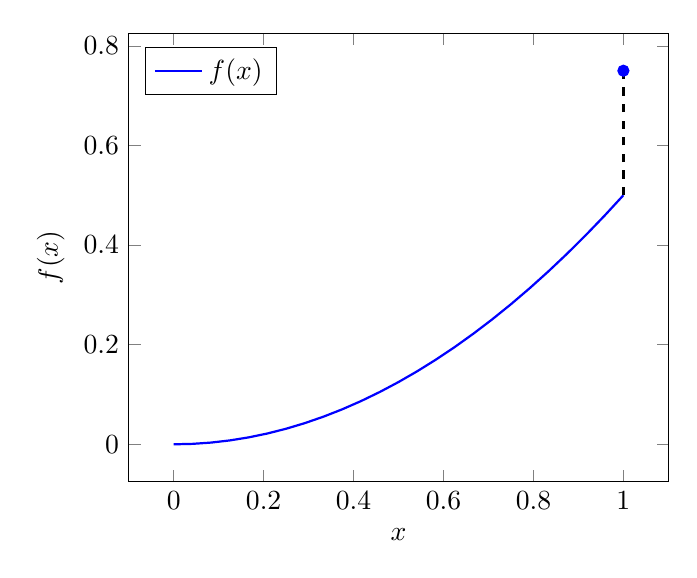
\begin{tikzpicture}% function
        \begin{axis}[xlabel=$x$,ylabel=$f(x)$, legend pos=north west]
        \addplot[thick, color=blue,domain = 0:1] {(0.5 * (x * x))};
        \addplot[mark=*, color=blue] coordinates {(1,0.75)};
        \draw [dashed, very thick] (1,0.5) -- (1,0.75);
        \legend{$f(x)$}
        \end{axis}
        \end{tikzpicture}
        \caption{Graph for $f$ from~\cref{eq:pw-f}}
        \label{fig:pw-f}
    \end{figure}
    \item $g$ is not necessarily closed. Take $\cC = \set{(x, y) \in \Rbb^2
        \mmid x^2 \leq y}$ and define
        \[
            f(x, y) = \begin{cases}
                0, & x = y = 0 \\
                x^2y^{-1}, & x \in \cC, y \neq 0.
            \end{cases}
        \]
        Take $\bar{x} = 0$. Obviously $g(0) = 0$ as we proved in the previous
        part of the problem. Now, consider $v_n = \begin{pmatrix}
        n^{-1/2} \\ n^{-1}
        \end{pmatrix}, \; n \geq 1$, which satisfies $0 + t v_n
        \in \dom f$ for small $t$, as $t^2 \frac{1}{n} \leq t \frac{1}{n}$.
        Then, the directional derivative is given by
        \[
            g(v_n) = \lim_{t \dto 0} \frac{\frac{t^2 n^{-1}}{t n^{-1}} -
            f(0)}{t}
            = \lim_{t \dto 0} \frac{t}{t} = 1.
        \]
        However, $v_n$ is a sequence of points approaching $(0, 0)$ as $n \to
        \infty$, for which $g(v_n) \overset{n \to \infty}{\to} 1 \neq g(0)$.
        Therefore, $g$ is not necessarily closed.
    \end{enumerate}
    The first of the examples above suffers from the fact that $f$ is originally
    not closed. Unfortunately, we were unable to find a counterexample for which
    $f$ is closed but $g$ is not proper. This is also reflected in the fact that
    we were not able to resolve the case where one of the directional
    derivatives could be $-\infty$ in the previous part of the question.
\end{Exercise}

\vspace{1em}

\begin{Exercise}
	We are given that $f$ is differentiable and convex, with $L$-Lipschitz
	gradient. This implies that
	\[
		\abs{\grad f(x) - \grad f(y)} \leq L \norm{x - y}.
	\]
	Additionally, we consider the sequence of points
	\begin{align}
		x_{k+1} = x_k - A_k^{-1} \grad f(x_k) \Rightarrow
		\grad f(x_k) = A_k \left(x_{k} - x_{k+1}\right)
		\label{eq:seq-def}
	\end{align}
	where $A_k$ is a sequence of symmetric matrices satisfying
	$\inf_k \underline{\lambda_k} > \frac{L}{2}, \; \sup_k \overline{\lambda_k}
	< \infty$, where $\underline{\lambda}_k$, $\overline{\lambda}_k$ are the
	smallest and largest eigenvalues of $A_k$, respectively.

	To prove that $\set{x_k}_{k=1}^{\infty}$ is a slope descent sequence, we
	need to verify the two postulates given in lecture. Let us try to verify
	the sufficient decrease condition first: we exploit the fact that $f$ is
	convex and $L$-smooth, which implies that it has the following quadratic
	upper bound:
	\begin{align}
		f(z) &\leq f(x) + \ip{\grad f(x), z - x} + \frac{L}{2} \norm{z - x}^2,
		\label{eq:quad-upper-bound},
	\end{align}
	which was stated in lecture and also proven in the lectures of ORIE 6328.
	If we set $x = x_k, z = x_{k+1}$ in~\cref{eq:quad-upper-bound}, we obtain
	(moving terms around):
	\begin{align*}
		f(x_k) - f(x_{k+1}) &\geq \ip{\grad f(x_k), x_{k} - x_{k+1}}
			- \frac{L}{2} \norm{x_k - x_{k+1}}^2 \\
			&\overset{\cref{eq:seq-def}}{=} \ip{A_k (x_{k} - x_{k+1}), x_k -
		x_{k+1}} - \frac{L}{2} \norm{x_k - x_{k+1}}^2 \Rightarrow \\
			&\geq \inf_k \underline{\lambda_k} \norm{x_k - x_{k+1}}^2
			- \frac{L}{2} \norm{x_k - x_{k+1}}^2,
	\end{align*}
	where we have made use of the variational definition of the smallest
	eigenvalue of a matrix:
	\[
		\underline{\lambda} = \inf_{d \neq 0} \frac{d^\top A d}{d^\top d}
		\Rightarrow d^\top A d \geq \underline{\lambda} \norm{d}^2, \; \forall
		d.
	\]
	Since $\inf_k \underline{\lambda}_k > \frac{L}{2}$, it must hold that
	$\exists \alpha > 0: \alpha = \inf_k \underline{\lambda}_k - \frac{L}{2}$,
	so that we may conclude
	\[
		f(x_k) - f(x_{k+1}) \geq \alpha \norm{x_k - x_{k+1}}^2, \; \forall k
		\in \Nbb,
	\]
	which is precisely the sufficient decrease condition. It remains to show
	that
	\[
		\abs{\grad f}(x_{k+1}) \leq \beta \norm{x_k - x_{k+1}}, \; \forall k.
	\]
	Notice that the Lipschitz bound along with the reverse triangle inequality
	give us
	\[
		\norm{\grad f(x_{k+1})} - \norm{\grad f(x_k)} \leq
		\norm{\grad f(x_{k+1}) - \grad f(x_k)} \leq L \norm{x_{k+1} - x_k}
	\]
	which, combined with~\eqref{eq:seq-def}, implies
	\begin{align*}
		\norm{\grad f(x_{k+1})} &\leq \norm{A_k (x_k - x_{k+1})} + L
		\norm{x_{k+1} - x_k} \leq \sup_k \overline{\lambda}_k \norm{x_{k+1} -
		x_k} + L \norm{x_{k+1} - x_k} \\
		&\leq \left(L + \lambda\right) \norm{x_{k+1} - x_k},
	\end{align*}
	where $\lambda = \sup_k \overline{\lambda}_k$, as our assumptions dictate
	that $\set{A_k}$ are uniformly bounded and $\norm{Ax} \leq \opnorm{A}
	\norm{x}$ when $\norm{\cdot} = \norm{\cdot}_2$. This completes the second
	postulate, since in Exercise 2 we proved that $\abs{\grad f}(x) =
	\norm{\grad f(x)}$ for a differentiable function $f$. Hence
	\[
		\abs{\grad f}(x_{k+1}) \leq \left(L + \lambda\right) \norm{x_{k+1} -
		x_k},
	\]
	and the sequence $\set{x_k}_{k=1}^{\infty}$ is indeed a slope descent
	sequence.
\end{Exercise}

\bibliographystyle{plain}
\bibliography{references}

\end{document}
